% ============================================================
% SECTION 1: BÀI TOÁN
% ============================================================
\section{Bài toán}

% --- Slide 1 ---
\begin{frame}{Bối cảnh}
\begin{columns}[T,onlytextwidth]
\begin{column}{0.5\textwidth}
\begin{itemize}
  \item Năm 2015: khoảng \textbf{5,8 triệu} chuyến bay nội địa Hoa Kỳ.
  \item Tỷ lệ đáng kể trễ đến $\geq 15$ phút,
        gây chi phí vận hành và giảm trải nghiệm hành khách.
  \item Phân tích thủ công (Excel, SQL rời rạc) \textbf{khó mở rộng},
        không phát hiện được pattern ẩn.
\end{itemize}

\vspace{2mm}
\begin{alertblock}{Nhu cầu}
Cần một hệ thống tích hợp: tự động hóa dữ liệu, phân tích đa chiều OLAP
\textbf{và} dự báo delay trước giờ cất cánh.
\end{alertblock}
\end{column}
\begin{column}{0.4\textwidth}
\centering

\includegraphics[width=1.1\linewidth]{plane.jpg}
\end{column}
\end{columns}
\end{frame}

% --- Slide 2 ---
\begin{frame}{Mục tiêu đề tài}
Ba mục tiêu cốt lõi:
\begin{enumerate}
  \item \textbf{Data Warehouse} theo Star Schema
  \begin{itemize}
    \item 1 bảng sự kiện (\texttt{fact\_flights}) + 4 bảng chiều.
    \item Pipeline ETL streaming theo chunk.
  \end{itemize}

  \item \textbf{Dashboard OLAP đa trang}
  \begin{itemize}
    \item 6 trang phân tích tương tác (Streamlit + Plotly).
    \item Hiện thực Slice, Dice, Roll-up, Drill-down.
  \end{itemize}

  \item \textbf{Mô hình dự báo delay}
  \begin{itemize}
    \item So sánh 5 thuật toán ML trên cùng pipeline.
    \item Đánh giá bằng 7 chỉ số, ưu tiên AUC-ROC.
  \end{itemize}
\end{enumerate}

\begin{block}{Đầu ra}
Dữ liệu thô $\rightarrow$ ETL $\rightarrow$ Kho dữ liệu $\rightarrow$ Dashboard + Mô hình dự báo.
\end{block}
\end{frame}

% --- Slide 3 ---
\begin{frame}{Nguồn dữ liệu}
Bộ dữ liệu công khai \textit{US Flight Delays 2015} (Kaggle):

\vspace{2mm}
\begin{table}
\centering
\small
\begin{tabular}{lrl}
\toprule
\textbf{Tệp} & \textbf{Số bản ghi} & \textbf{Nội dung} \\
\midrule
\texttt{flights.csv}  & 5.819.079 & 31 thuộc tính chuyến bay \\
\texttt{airlines.csv}  & 14 & Hãng hàng không nội địa \\
\texttt{airports.csv}  & 322 & Sân bay, vị trí, tọa độ \\
\bottomrule
\end{tabular}
\end{table}

\vspace{2mm}
\textbf{Phạm vi:} Chuyến bay nội địa Hoa Kỳ từ 01/01 đến 31/12/2015.
Không bao gồm chuyến bay quốc tế hoặc dữ liệu thời tiết thực tế.
\end{frame}

% --- Slide 4 ---
\begin{frame}{Thách thức chính}
\begin{columns}[T,onlytextwidth]
\begin{column}{0.45\textwidth}
\begin{enumerate}
  \item \textbf{Giá trị thiếu có cấu trúc}
  \begin{itemize}
    \item $\approx$76\% bản ghi thiếu chi tiết delay thành phần.
    \item Cột delay trống khi chuyến bị hủy hoặc chuyển hướng.
  \end{itemize}

  \item \textbf{Mất cân bằng lớp}
  \begin{itemize}
    \item $\approx$81\% đúng giờ vs. 19\% trễ.
    \item Imbalance ratio $\approx$ 4,23:1.
  \end{itemize}

  \item \textbf{Rò rỉ tương lai}
  \begin{itemize}
    \item \texttt{departure\_delay} chỉ biết \textit{sau} khi rời cổng.
    \item Phải loại để đảm bảo tính ``dự báo''.
  \end{itemize}
\end{enumerate}
\end{column}
\begin{column}{0.5\textwidth}
\centering
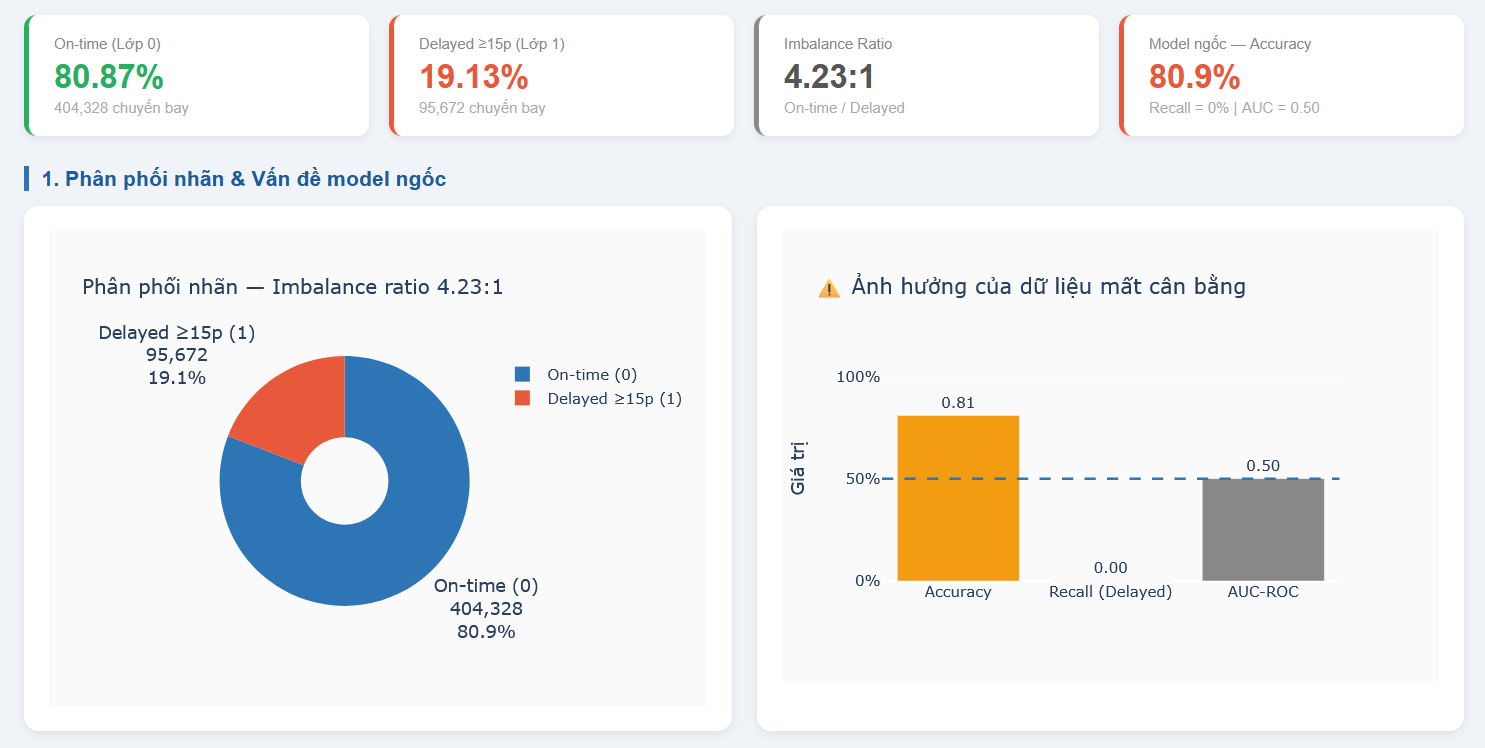
\includegraphics[width=\linewidth,height=0.65\textheight,keepaspectratio]{imbalance_analysis.png}
\end{column}
\end{columns}
\end{frame}
